\documentclass[aspectratio=169, 12pt]{beamer}

\usetheme{Madrid}

\definecolor{tealblue}{HTML}{0D6E82}
\definecolor{mygray}{HTML}{7F8C8D}
\definecolor{myorange}{HTML}{E67E22}
\definecolor{placeholderbg}{HTML}{D5D8DC}

\usecolortheme{default}

\usepackage{amsmath, amssymb}
\usepackage{booktabs}
\usepackage{colortbl}
\usepackage{xcolor}
\usepackage{graphicx}
\usepackage{tikz}
\usetikzlibrary{shapes.geometric, arrows.meta, positioning, backgrounds}
\usepackage{array}
\usepackage{multirow}

% Placeholder command: \imgplaceholder{width}{height}{label}
\newcommand{\imgplaceholder}[3]{%
  \begin{tikzpicture}
    \fill[placeholderbg] (0,0) rectangle (#1,#2);
    \draw[mygray, dashed, thick] (0,0) rectangle (#1,#2);
    \node[mygray, font=\small\itshape, align=center, text width=#1 cm]
      at ({#1/2},{#2/2}) {#3};
  \end{tikzpicture}%
}

\title{Pixel vs Symbolic Observations for PPO}
\subtitle{Super Mario Bros Reinforcement Learning}
\author{Lucas Martim \and Sergio Contente \and Leonardo Falabella \and Gabriel Corsi \and Lara Polachini}
\institute{CSC-52081 --- Reinforcement Learning}
\date{\today}

\begin{document}

\begin{frame}
\titlepage
\end{frame}

\begin{frame}{Outline}
\tableofcontents
\end{frame}

%================================================
\section{Motivation}
%================================================

\begin{frame}{Motivation}
\begin{columns}[T]
\column{0.50\textwidth}
\textbf{Why Mario?}
\begin{itemize}
  \item Classic RL benchmark
  \item Semi-Sparse rewards, precise control
  \item High-dimensional pixel observations
\end{itemize}

\vspace{8pt}
\textbf{Our question:}\\
Can \emph{symbolic} (RAM-based) state + PPO\\
beat pixel-based DQN?

\column{0.46\textwidth}
\begin{center}
  
\includegraphics[width=0.9\linewidth]{images/mario_cape.png}
\end{center}
\end{columns}
\end{frame}

%================================================
\section{Project Overview}
%================================================

\begin{frame}{Project Overview}
\begin{columns}[T]
\column{0.50\textwidth}
\textbf{Experiments, in order:}
\begin{enumerate}
  \item DQN baseline (symbolic obs.)
  \item Pixel PPO (CNN)
  \item Symbolic PPO (RAM grid)
  \item Transfer: World 1-1 $\to$ 1-2
  \item Multi-task: From 1-1 to 1-4 jointly
  \item Random start positions
\end{enumerate}

\column{0.46\textwidth}
\begin{block}{Two observation types}
\small
\begin{tabular}{ll}
  \toprule
  \textbf{Pixel} & Raw frames + CNN \\
  \textbf{Symbolic} & NES RAM $\to$ tile grid \\
  \bottomrule
\end{tabular}
\end{block}
\vspace{6pt}
\begin{exampleblock}{}
\small
RAM = structured \& compact,\\
but requires domain knowledge.
\end{exampleblock}
\end{columns}
\end{frame}

% %================================================
% \section{Background}
% %================================================

% \begin{frame}{Background: DQN}
% \[
%   \mathcal{L}(\theta)= \mathbb{E}\!\left[\bigl(r + \gamma \max_{a'} Q(s',a';\theta^{-}) - Q(s,a;\theta)\bigr)^2\right]
% \]

% \vspace{6pt}
% Trained on symbolic obs.\ for $2\,$M steps.

% \vspace{6pt}
% \begin{alertblock}{Result: 0\% flag rate}
% \begin{itemize}
%   \item $\varepsilon$-greedy disrupts sustained action sequences
%   \item Replay buffer fills with correlated failures
%   \item Noisy $Q$-targets destabilise learning
% \end{itemize}
% \end{alertblock}
% \end{frame}

% %------------------------------------------------
% \begin{frame}{Background: PPO}
% \[
%   \mathcal{L}^{\text{CLIP}}(\theta)=
%   \mathbb{E}_t\!\left[\min\!\left(r_t(\theta)\,\hat{A}_t,\;
%   \operatorname{clip}(r_t(\theta),1\!-\!\epsilon,1\!+\!\epsilon)\,\hat{A}_t\right)\right]
% \]

% \begin{columns}[T]
% \column{0.47\textwidth}
% \begin{block}{Why PPO works here}
% \small
% \begin{itemize}
%   \item On-policy: no stale replay buffer
%   \item $N=8$ parallel envs $\to$ diverse transitions
%   \item GAE propagates sparse rewards
% \end{itemize}
% \end{block}

% \column{0.47\textwidth}
% \begin{block}{Key hyperparameters}
% \footnotesize
% \begin{tabular}{lr}
%   \toprule
%   $\gamma$ & $0.90$ \\
%   lr Phase 1 / 2 & $2.5\!\times\!10^{-4}$ / $10^{-5}$ \\
%   Steps, batch & $512$, $256$ \\
%   Clip $\epsilon$, entropy & $0.1$, $0.01$ \\
%   \bottomrule
% \end{tabular}
% \end{block}
% \end{columns}
% \end{frame}

%================================================
\section{Methodology}
%================================================

\begin{frame}{Methodology: Observations}
\begin{columns}[T]
\column{0.48\textwidth}
\begin{block}{Pixel}
\begin{itemize}
  \item $84\!\times\!84$ grayscale, 4 stacked frames
  \item Nature CNN $\to$ FC 512
  \item \textbf{78 FPS} on Colab T4
\end{itemize}
\end{block}

\vspace{6pt}
\begin{center}
  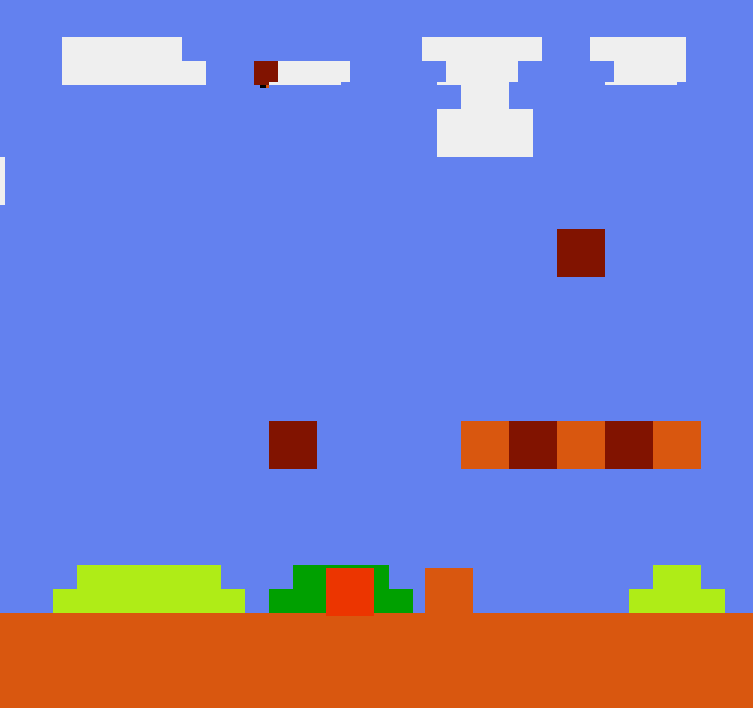
\includegraphics[width=0.5\linewidth]{images/pixel.png}
\end{center}

\column{0.48\textwidth}
\begin{block}{Symbolic (RAM)}
\begin{itemize}
  \item $13\!\times\!16$ tile grid, 4 stacked
  \item Encodes: terrain, enemies, Mario
  \item MLP [512, 512]
  \item \textbf{500 FPS} on CPU
\end{itemize}
\end{block}

\vspace{6pt}
\begin{center}
  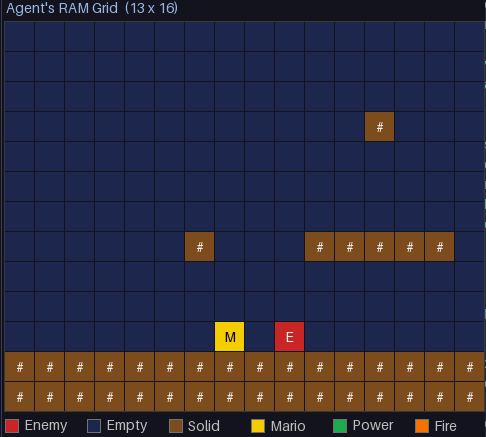
\includegraphics[width=0.5\linewidth]{images/ram.png}
\end{center}
\end{columns}
\end{frame}

%------------------------------------------------
\begin{frame}{Methodology: Reward Shaping}
\[
  r \;\leftarrow\; \frac{1}{10}\!\left[
      r_{\text{env}}
      + \frac{\Delta\text{score}}{40}
      + 50\cdot\mathbf{1}[\text{flag}]
      - 50\cdot\mathbf{1}[\text{death}]
  \right]
\]

\begin{itemize}
  \item $r_{\text{env}}$: horizontal progress
  \item $\Delta\text{score}/40$: coins, kills, blocks
  \item $\pm50$: flag bonus / death penalty
  \item $\div 10$: normalises reward scale
\end{itemize}
\end{frame}

%================================================
\section{Results}
%================================================

\begin{frame}{Results: World 1-1 Summary}
\begin{alertblock}{Symbolic DQN --- 0\% flag}
  Never escapes the first obstacle.
\end{alertblock}
\vspace{6pt}
\begin{block}{Pixel PPO --- $>$80\% flag}
  Mean reward $\approx 285$.\quad Slow: 78 FPS on GPU.
\end{block}
\vspace{6pt}
\begin{exampleblock}{Symbolic PPO --- 93\% flag (peak 97\%)}
  Mean reward $\approx 304$.\quad Fast: 500 FPS on CPU.
\end{exampleblock}
\end{frame}

%------------------------------------------------
\begin{frame}{Results: World 1-1 Summary (Training Curves)}
\begin{center}
  \includegraphics[width=0.85\linewidth]{images/ppo_pixel_symbol_dqn_w1l1.png}
\end{center}
\end{frame}

%------------------------------------------------
\begin{frame}{Results: Transfer Learning 1-1 $\to$ 1-2}
\begin{columns}[T]
\column{0.32\textwidth}
\begin{block}{Setup}
\small
Train on 1-1 $\to$ fine-tune on 1-2\\
(lr $= 10^{-5}$, weights unfrozen)
\end{block}
\column{0.32\textwidth}
\begin{exampleblock}{World 1-2: \textbf{78\% flag rate}}
\small Converges faster than from scratch.
\end{exampleblock}
\column{0.32\textwidth}
\begin{alertblock}{World 1-1: \textbf{0\% flag rate}}
\small Complete performance collapse.
\end{alertblock}
\end{columns}
\vspace{4pt}
\begin{center}
  \includegraphics[width=0.8\linewidth]{images/symbolic/comparison_w1l1_w1l2_ppo/catastophic.png}
\end{center}
\end{frame}

%------------------------------------------------
\begin{frame}{Results: Random-Start Curriculum (World 1-1)}
\begin{columns}[T]
\column{0.52\textwidth}
\textbf{Problem:} fixed start $\Rightarrow$ agent memorises one trajectory.

\vspace{6pt}
\textbf{Two-layer solution:}
\begin{enumerate}
  \item \textbf{Random-start wrapper} --- at each reset, execute
        $n \sim \mathcal{U}[0, N_{\max}]$ forward actions\\
        {\small(right / right+A / right+B / right+A+B)}\\
        Mario \emph{walks} into the level, not teleported.
  \item \textbf{Curriculum callback} --- linearly anneal
        $N_{\max}: 0 \to 100$ over training (every 1\,k steps). Easy start first, then harder as the agent improves.
\end{enumerate}

\vspace{6pt}
\begin{exampleblock}{Result}
Agent generalises across all level sections;\\
stable flag rate from any start position.
\end{exampleblock}

\column{0.44\textwidth}
\begin{block}{Design separation}
\small
\begin{tabular}{p{1.6cm}p{2.5cm}}
  \toprule
  \textbf{Random start} & \emph{how} Mario is placed \\
  \textbf{Curriculum}   & \emph{when/how far} to place him \\
  \bottomrule
\end{tabular}
\end{block}
\end{columns}
\end{frame}

%------------------------------------------------
\begin{frame}{Results: Multi-Task (Worlds 1-1 to 1-4)}
\begin{columns}[T]
\column{0.50\textwidth}
\textbf{Setup:} Worlds 1-1 through 1-4, shared PPO policy.

\vspace{8pt}
\begin{alertblock}{Problem: reward imbalance}
1-1 yields rewards earliest $\Rightarrow$\\
its gradients dominate $\Rightarrow$\\
later worlds stagnate.
\end{alertblock}

\vspace{6pt}
{\small\textit{Fix:} per-task reward normalisation or gradient surgery \cite{Yu2020}.}

\column{0.46\textwidth}
\begin{center}
  \imgplaceholder{5.2}{4.2}{Multi-task curves\\(W1-1 through W1-4 flag rates)}
\end{center}
\end{columns}
\end{frame}

%================================================
\section{Discussion \& Conclusion}
%================================================

\begin{frame}{Discussion}
\begin{columns}[T]
\column{0.50\textwidth}
\textbf{Key takeaways:}
\begin{enumerate}
  \item Algorithm $>$ representation:\\
        same obs., DQN fails, PPO succeeds
  \item Symbolic = $6\times$ faster wall-clock,\\
        higher peak performance
  \item On-policy transfer $\to$ catastrophic forgetting
  \item Multi-task needs reward balancing
\end{enumerate}

\column{0.46\textwidth}
\begin{block}{Trade-off}
\small
\begin{tabular}{p{1.5cm}p{2.8cm}}
  \toprule
  \textbf{Pixel}    & General, no domain knowledge \\
  \textbf{Symbolic} & Fast, compact, but fragile \\
  \bottomrule
\end{tabular}
\end{block}
\end{columns}
\end{frame}

%------------------------------------------------
\begin{frame}{Conclusion}
\begin{columns}[T]
\column{0.50\textwidth}
\textbf{Contributions:}
\begin{itemize}
  \item PPO strongly outperforms DQN on Mario
  \item Symbolic states: $6\times$ speedup, better reward
  \item Empirical study of catastrophic forgetting
  \item Reward imbalance identified as multi-task bottleneck
\end{itemize}

\end{columns}
\end{frame}

% REFERENCES
\begin{frame}[allowframebreaks]{References}
\footnotesize
\begin{thebibliography}{99}
\bibitem{Schulman2017} J.~Schulman et al.\ \emph{PPO Algorithms}. arXiv:1707.06347, 2017.
\bibitem{Mnih2015} V.~Mnih et al.\ \emph{Human-level control via DRL}. Nature, 518, 2015.
\bibitem{Raffin2021} A.~Raffin et al.\ \emph{Stable-Baselines3}. JMLR, 22(268), 2021.
\bibitem{McCloskey1989} M.~McCloskey, N.~J.~Cohen. \emph{Catastrophic Interference}. Psych.\ Learning \& Motivation, 24, 1989.
\bibitem{Kirkpatrick2017} J.~Kirkpatrick et al.\ \emph{Overcoming Catastrophic Forgetting}. PNAS, 114(13), 2017.
\bibitem{Yu2020} T.~Yu et al.\ \emph{Gradient Surgery for MTL}. NeurIPS, 2020.
\end{thebibliography}
\end{frame}

\begin{frame}
\begin{center}
  \vspace{1cm}
  {\Huge\textbf{Thank You}}\\[12pt]
  {\large\textcolor{red}{Questions?}}\\[20pt]
  {\small Lucas Martim $\cdot$ Sergio Contente $\cdot$ Leonardo Falabella $\cdot$ Gabriel Corsi $\cdot$ Lara Polachini}\\[8pt]
  {\footnotesize CSC-52081 $\cdot$ Reinforcement Learning $\cdot$ March 2026}
\end{center}
\end{frame}

\end{document}
